\documentclass[mathserif,handout]{beamer}

% packages
\usepackage{physics}
\usepackage{amsfonts, amsmath, amssymb, amsthm}
\usepackage{graphicx}
\usepackage[mathscr]{euscript}
\usepackage{xcolor}
\usepackage{comment}
\usepackage{tikz}

\usetheme{Warsaw}

\definecolor{GTtechgold}{RGB}{167,147,75}
\definecolor{GTbuzzgold}{RGB}{234,170,0}
\definecolor{GTbuzzgold60}{RGB}{245,213,128}
\definecolor{GTblue}{RGB}{0,48,87}
\definecolor{GTdarkgrey}{RGB}{84,84,84}
\definecolor{GTpalettedark}{RGB}{84,88,90}
\definecolor{GTpalettemed}{RGB}{142,139,118}
\definecolor{GTpalettelight}{RGB}{214,219,212}

\usecolortheme[named=GTtechgold]{structure}
\setbeamercolor{title}{bg=GTpalettelight,fg=}

\setbeamercolor{frametitle}{bg=GTblue,fg=GTpalettelight}

\setbeamercolor{palette primary}{bg=GTpalettelight,fg=GTblue}
\setbeamercolor{palette secondary}{bg=GTpalettemed,fg=white}
\setbeamercolor{palette tertiary}{bg=GTblue,fg=GTtechgold}
\setbeamercolor{palette quaternary}{bg=GTpalettelight,fg=GTblue}

% block colors
\BeforeBeginEnvironment{theorem}{%
    \setbeamercolor{block title}{fg=white,bg=GTblue}
}
\AfterEndEnvironment{theorem}{
        \setbeamercolor{block title}{use=structure,fg=white,bg=structure.fg!75!black}
}

\BeforeBeginEnvironment{definition}{%
    \setbeamercolor{block title}{fg=white,bg=GTpalettedark}
}
\AfterEndEnvironment{definition}{
        \setbeamercolor{block title}{use=structure,fg=white,bg=structure.fg!75!black}
}

% To get page numbers:
\setbeamertemplate{footline}[frame number]

% paragraph indentation/spacing
\setlength{\parindent}{0cm}
\setlength{\parskip}{5pt}
\renewcommand{\baselinestretch}{1.25}

\newcommand{\br}[1]{\left(#1\right)}
\newcommand{\sbr}[1]{\left[#1\right]}
\newcommand{\cbr}[1]{\left\{#1\right\}}
\newcommand{\pr}{\mathfrak P}
\newcommand{\vect}[1]{\mathbf#1}
\newcommand{\Z}{\mathbb Z}
\newcommand{\Prj}{\mathbb P}
\newcommand{\R}{\mathbb R}
\newcommand{\N}{\mathbb N}

\DeclareMathOperator{\Cone}{Cone}
\DeclareMathOperator{\Spec}{Spec}
\DeclareMathOperator{\Hom}{Hom}
\DeclareMathOperator{\im}{im}
\DeclareMathOperator{\cone}{cone}

\title
{\color{GTblue}{Toric varieties given by principal 2-minor ideals}}

\subtitle{Undergraduate Mathematics Research Symposium 2023}

\author[Sai Sivakumar]
{Sai Sivakumar}

\institute[Georgia Tech]{\color{GTtechgold}{University of Florida}}
\date{28 April 2023}

\begin{document}

%The next statement creates the title page.
\frame{\titlepage}

\begin{frame}{}{}
{\color{GTtechgold}Thank you for inviting me to speak!}
\vspace{0.75pc}
\hrule
\vspace{0.75pc}
This is joint work with Erick Boniface (NC State), Andrew Rodriguez (Baruch College), and Dr. Ashley Wheeler (Georgia Tech).

\vspace{0.75pc}
This project arose from the Georgia Tech REU 2022. 
\end{frame}

% % % % %
%\section{Introduction}

% % % 
\begin{frame}{Introduction}
Let $K$ be an algebraically closed field and $X=(x_{ij})$ an $n\times n$ matrix of variables.


\vspace{0.75pc} 
\begin{definition}
    A \textbf{principal $t$-minor} of $X$ is the determinant of a $t\times t$ submatrix of $X$ whose row and column indices are the same; i.e., the submatrix is symmetric about the main diagonal of $X$.
\end{definition}

We have a \textbf{principal $t$-minor ideal} $\pr_t$ in the polynomial ring $K[x_{11},\dots,x_{ij},\dots,x_{nn}]$, which is generated by the principal $t$-minors of $X$. 
\end{frame}

% % % 
\begin{frame}
In this project, we are particularly interested in $\pr_2$.

\vspace{0.75pc}
\begin{block}{Example}
    For $n =2$, we have $\pr_2 = \langle x_{11}x_{22}-x_{12}x_{21}\rangle$.
\end{block}

\vspace{0.75pc}
\begin{definition}
    A \textbf{toric variety} is an irreducible variety $V$ that contains an algebraic torus as a Zariski open subset, such that the group action of the torus on itself extends to an action on $V$.
\end{definition}

\end{frame}

% % %
\begin{frame}
A \textbf{toric ideal} is an ideal which is prime and is generated by binomials. The vanishing set of a toric ideal is a toric variety. 

\vspace{0.75pc}
\begin{theorem}[Ene+Qureshi 2013, W 2015]
The ideal $\pr_2$ is toric, that is, it is prime and generated by binomials.
\end{theorem}  

So the vanishing set of $\pr_2$ is a toric variety.
\end{frame}

% % % % %
%\section{Monomial maps}

% % % 
\begin{frame}{Monomial maps}
Toric varieties can be defined using a monomial map of an algebraic torus.

 
\vspace{0.75pc}
Let $\mathscr A=\{\vect m_1,\dots,\vect m_s\}\subseteq \Z^d$ and define the map
\begin{align*}
\Phi_{\mathscr A}: (K^*)^d &\to K^s \\
\vect t &\mapsto (\vect t^{\vect m_1},\dots,\vect t^{\vect m_s})
\end{align*}
where for $\vect t=(t_1,\dots,t_d)\in (K^*)^d$ and $\vect m=(a_1,\dots,a_d)\in \Z^d$, $\vect t^{\vect m}=t_1^{a_1}\cdots t_d^{a_d}$.
\end{frame}

% % % 
\begin{frame}
The \textbf{affine toric variety} $Y_{\mathscr A}$ is the Zariski closure in $K^s$ of the image of $\Phi_{\mathscr A}$, which is its torus.


\vspace{0.75pc}
The \textbf{projective toric variety} $X_{\mathscr A}$ is the Zariski closure of the image of the composition map (which is its torus)
\[(K^\ast)^d\xrightarrow{\Phi_{\mathscr{A}}}K^s\xrightarrow{\eta}\Prj^{s-1},\]
where $\eta$ is the quotient map $\eta: K^s\to (K^s\setminus \{\vect 0\})/K^*=\Prj^{s-1}$.
\end{frame}

% % %
\begin{frame}
Since $\pr_2$ is homogeneous, the algebraic set $V(\pr_2)$ can be viewed as an affine or projective toric variety.  In this talk we will mainly regard $V(\pr_2)$ as an affine toric variety.  

\vspace{0.75pc}
We determined the finite set $\mathscr A$ of integer vectors that gives the monomial map defining $V(\pr_2)$. 
\end{frame}

% % % 
\begin{frame}
\setbeamercolor{block title}{fg=white,bg=GTpalettedark}
\begin{block}{Notation}
For vectors in $\binom{n+1}{2}$ dimensions, we use the indexing $11,12,\dots,$ $1n,22,\dots 2n,\dots,nn$ for their components.
\end{block}

\setbeamercolor{block title}{fg=white,bg=GTblue}
\begin{block}{Proposition [BRSW]}
$\vect I(Y_{\mathscr A_n})=\vect I(X_{\mathscr A_n})=\pr_2$, where 
\begin{multline*}
\mathscr A_n = \{\vect e_{ij}\mid 1\leq i\leq j\leq n\} \\
\cup \{\vect e_{ii}-\vect e_{ij}+\vect e_{jj}\mid 1\leq i\leq j\leq n\}\subseteq \Z^{\binom{n+1}{2}}.
\end{multline*}
\end{block}
\end{frame}

% % % 
\begin{frame}
%\vspace{0.75pc}
\begin{block}{Example}
For $n=2$ we have 
%\[
$\mathscr A_2 = \{\vect e_{11},\vect e_{12},\vect e_{22},\vect e_{11}-\vect e_{12}+\vect e_{22}\}\subseteq\Z^3
$ %\]
and the monomial map
\begin{align*}
\Phi_{\mathscr A_2}: (K^*)^3 &\to (K^*)^4\subseteq K^4 \\
(t_{11},t_{12},t_{22}) &\mapsto (t_{11},t_{12},t_{22},t_{11}t_{12}^{-1}t_{22}).
\end{align*} Furthermore, 
\[
\vect I(Y_{\mathscr A_2})= \langle x_{11}x_{22}-x_{12}x_{21}\rangle=\pr_2=\vect I(X_{\mathscr A_2}).
\]
\end{block}
\end{frame}

% % % % % 
%\section{Cones}% and affine toric varieties}

% % % 
\begin{frame}
{Cones}% and affine toric varieties}
So far we have two ways to describe an affine toric variety in $K^s$:


\begin{enumerate}[]
\item The vanishing set of a toric ideal


\item The Zariski closure of the monomial map $\Phi_{\mathscr{A}}$ for a finite set $\mathscr A\subseteq \Z^d$.
\end{enumerate}


%\vspace{0.75pc}
We now illustrate a third way to describe an affine toric variety, using cones.
\end{frame}

% % %
\begin{frame}
The torus $T=\im(\Phi_{\mathscr A})\subseteq Y_{\mathscr A}$ comes equipped with dual lattices $M=\Z\mathscr A$ and $N=\Hom_{\Z}(M,\Z)$, both with rank equal to $\dim T$.

\vspace{0.75pc}
$Y_{\mathscr A}$ can be described as $\Spec K[S_{\sigma}]$ for some rational polyhedral cone $\sigma\subseteq N_{\R}=N\otimes_{\Z}\R$.
    

\end{frame}

% % %
\begin{frame}
    $S_{\sigma}=\sigma^{\vee}\cap M$, where $\sigma^{\vee}$ is the \textbf{dual cone} of $\sigma$:
    \[
    \sigma^{\vee} = \{\vect m\in M\otimes_{\Z}\R\mid \langle \vect m,\vect u\rangle\geq 0 \text{ for all $\vect u\in\sigma$}\}.
    \]
    
    $K[S_{\sigma}]\subseteq K[x_1^{\pm 1},\dots,x_d^{\pm 1}]$ is the $K$-subalgebra generated by monomials whose exponent vectors are in $S_{\sigma}$.
\end{frame}

% % %
\begin{frame}
    \begin{columns}
        \begin{column}{0.5\textwidth}
            \begin{theorem}[BRSW]
                Let \[\sigma_n^{\vee} = \cone(\mathscr A_n)\]
                \begin{multline*}
                    = \bigg\{\sum_{\vect m\in\mathscr A_n}\lambda_{\vect m}\vect m\ \bigg|\  \lambda_{\vect m}\geq 0\bigg\}.
                \end{multline*}
                Then $\sigma_n=(\sigma_n^{\vee})^{\vee}$ is strongly convex and rational.  Therefore, $\Spec K[S_{\sigma_n}]$ is normal. 
            \end{theorem}
        \end{column}
        \begin{column}{0.5\textwidth}
            \begin{block}{Example (n=2)}
                The cone $\sigma^\vee_2 = \cone(\mathscr{A}_2)$:\begin{center}
                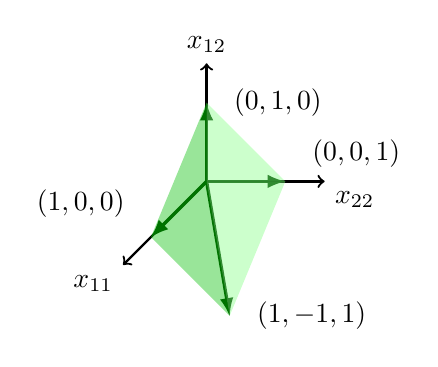
\begin{tikzpicture}%
                    [x={(-0.707106cm, -0.707106cm)},
                    y={(1cm, 0cm)},
                    z={(0cm, 1cm)},
                    scale=1.00000,
                    back/.style={loosely dotted, thin},
                    edge/.style={color=blue!50!black, very thick},
                    facet/.style={fill=green!50!white,fill opacity=0.400000},
                    facet2/.style={fill=green!75!black,fill opacity=0.400000},
                    vertex/.style={inner sep=1pt,circle,draw=blue!50!black,fill=blue!50!black,thick}]
            
                %% Drawing the axes
                \draw[color=black,thick,->] (0,0,0) -- (1.5,0,0) node[anchor=north east]{$x_{11}$};
                \draw[color=black,thick,->] (0,0,0) -- (0,1.5,0) node[anchor=north west]{$x_{22}$};
                \draw[color=black,thick,->] (0,0,0) -- (0,0,1.5) node[anchor=south]{$x_{12}$};
                %% Rays for cone:   
                \draw[color=green!25!black,very thick,-latex] (0,0,0)--(0,0,1);
                \draw[color=green!25!black,very thick,-latex] (0,0,0)--(0,1,0);
                \draw[color=green!25!black,very thick,-latex] (0,0,0)--(1,0,0);
                \draw[color=green!25!black,very thick,-latex] (0,0,0)--(1,1,-1);
                %%
                %% Drawing the interior
                %%
                \fill[facet] (0, 0, 0) -- (0, 1, 0) -- (0, 0, 1) -- (0, 0, 0) -- cycle {};
                \fill[facet] (0,0,0) -- (1, 1, -1) -- (0, 1, 0) -- (0, 0, 0) -- cycle {};
                \fill[facet2] (0,0,0) -- (1,0,0) -- (1, 1, -1) -- (0, 0, 0) -- cycle {};
                \fill[facet2] (0, 0, 0) -- (1, 0, 0) -- (0, 0, 1) -- (0, 0, 0) -- cycle {};
                %%
                %% Drawing the vertices
                %%
                \node[label={[label distance=0.1cm]0:$(0,1,0)$}] at (0.00000, 0.00000, 1.00000)    {};
                \node[label={[label distance=0.1cm]15:$(0,0,1)$}] at (0.00000, 1.00000, 0.00000)     {};
                \node[label={[label distance=0.1cm]150:$(1,0,0)$}] at (1.00000, 0.00000, 0.00000)     {};
                \node[label={[label distance=0.1cm]0:$(1,-1,1)$}] at (1.00000, 1.00000, -1.00000)     {};
                %%
                %%
                \end{tikzpicture}
            \end{center}
            \end{block}
        \end{column}
    \end{columns}
    \vspace{0.75pc}
    It can be shown that $Y_{\mathscr A_n}\cong\Spec K[S_{\sigma_n}]$.
\end{frame}

% % % 
\begin{frame}
\begin{theorem}[BRSW]
If $\sigma_n^{\vee}=\cone(\mathscr A_n)$ then $\sigma_n = (\sigma_n^{\vee})^{\vee} = \cone(\mathscr B_n)$, where $\mathscr B_n=\cup_{i=1}^n\mathscr B_n^i$ and 
\[
\mathscr B_n^i\!=\!\bigg\{\vect e_{ii} + \sum_{\vect e \in E} \vect e \ \bigg|\ E \subseteq \{\vect e_{1i},\ldots,\vect e_{i-1,i},\vect e_{i,i+1} \ldots,\vect e_{in}\}\bigg\}\subseteq \Z^{\binom{n+1}{2}}
\]
\end{theorem}


\begin{block}{Example (n=2)}
    \begin{columns}
        \begin{column}{4.75cm}
            We have $\mathscr B_2 = \{\vect e_{11},\vect e_{11}+\vect e_{12}, \vect e_{22}, \vect e_{12}+\vect e_{22}\}$. Depicted is $\sigma_2 =\cone(\mathscr{B}_2)$:
        \end{column}
        \begin{column}{5cm}
            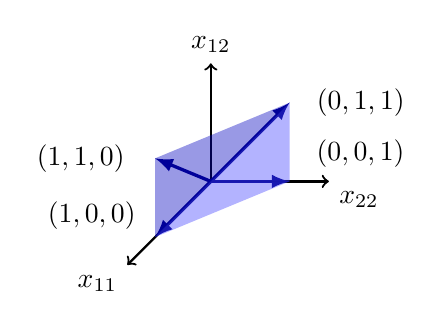
\begin{tikzpicture}%
                [x={(-0.707106cm, -0.707106cm)},
                y={(1cm, 0cm)},
                z={(0cm, 1cm)},
                scale=1.000000,
                back/.style={loosely dotted, thin},
                edge/.style={color=blue!50!black, very thick},
                facet/.style={fill=blue!75!white,fill opacity=0.400000},
                facet2/.style={fill=blue!75!black,fill opacity=0.400000},
                vertex/.style={inner sep=1pt,circle,draw=blue!50!black,fill=blue!50!black,thick}]
        
            %% Drawing the axes
            \draw[color=black,thick,->] (0,0,0) -- (1.5,0,0) node[anchor=north east]{$x_{11}$};
            \draw[color=black,thick,->] (0,0,0) -- (0,1.5,0) node[anchor=north west]{$x_{22}$};
            \draw[color=black,thick,->] (0,0,0) -- (0,0,1.5) node[anchor=south]{$x_{12}$};
            %% Rays for cone:   
            \draw[color=blue!50!black,very thick,-latex] (0,0,0)--(1,0,1);
            \draw[color=blue!50!black,very thick,-latex] (0,0,0)--(0,1,0);
            \draw[color=blue!50!black,very thick,-latex] (0,0,0)--(1,0,0);
            \draw[color=blue!50!black,very thick,-latex] (0,0,0)--(0,1,1);
            %%
            %% Drawing the interior
            %%
            \fill[facet] (0, 0, 0) -- (0, 1, 0) -- (0, 1, 1) -- (0, 0, 0) -- cycle {};
            \fill[facet2] (0,0,0) -- (0, 1, 1) -- (1, 0, 1) -- (0, 0, 0) -- cycle {};
            \fill[facet2] (0,0,0) -- (1,0,1) -- (1, 0, 0) -- (0, 0, 0) -- cycle {};
            \fill[facet] (0, 0, 0) -- (1, 0, 0) -- (0, 1, 0) -- (0, 0, 0) -- cycle {};
            %%
            %% Drawing the vertices
            %%
            \node[label={[label distance=0.1cm]0:$(0,1,1)$}] at (0.00000, 1.00000, 1.00000)    {};
            \node[label={[label distance=0.1cm]15:$(0,0,1)$}] at (0.00000, 1.00000, 0.00000)     {};
            \node[label={[label distance=0cm]150:$(1,0,0)$}] at (1.00000, 0.00000, -0.100000)     {};
            \node[label={[label distance=-1.75cm]0:$(1,1,0)$}] at (1.00000, 0.00000, 1.00000)     {};
            %%
            %%
            \end{tikzpicture}
        \end{column}
    \end{columns}

\end{block}
\end{frame}

% % %
\begin{frame}{The projective toric variety $X_{\mathscr A_n}$}
\begin{columns}
    \begin{column}{0.5\textwidth}
        We showed the dimension of the lattice polytope $P_n$ associated to $X_{\mathscr A_n}$ is equal to $\binom{n+1}{2}-1$.
        \begin{center}
            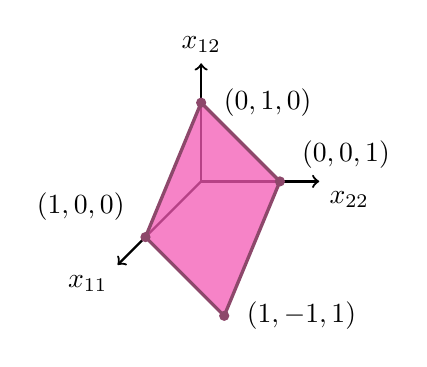
\begin{tikzpicture}%
                [x={(-0.707106cm, -0.707106cm)},
                y={(1cm, 0cm)},
                z={(0cm, 1cm)},
                scale=1.00000,
                back/.style={loosely dotted, thin},
                edge/.style={color=magenta!50!black, very thick},
                facet/.style={fill=magenta!65!white,fill opacity=0.750000},
                vertex/.style={inner sep=1pt,circle,draw=magenta!50!black,fill=magenta!50!black,thick}]
            %
            %
            %% This TikZ-picture was produced with Sagemath version 9.6
            %% with the command: ._tikz_2d_in_3d and parameters:
            %% view = [-0.124500000000000, -0.300500000000000, -0.945600000000000]
            %% angle = 145
            %% scale = 2
            %% edge_color = orange
            %% facet_color = orange
            %% opacity = 0.400000000000000
            %% vertex_color = blue
            %% axis = True
            
            %% Drawing the axes
            \draw[color=black,thick,->] (0,0,0) -- (1.5,0,0) node[anchor=north east]{$x_{11}$};
            \draw[color=black,thick,->] (0,0,0) -- (0,1.5,0) node[anchor=north west]{$x_{22}$};
            \draw[color=black,thick,->] (0,0,0) -- (0,0,1.5) node[anchor=south]{$x_{12}$};
            %% Coordinate of the vertices:
            %%
            \coordinate (0.00000, 0.00000, 1.00000) at (0.00000, 0.00000, 1.00000);
            \coordinate (0.00000, 1.00000, 0.00000) at (0.00000, 1.00000, 0.00000);
            \coordinate (1.00000, 0.00000, 0.00000) at (1.00000, 0.00000, 0.00000);
            \coordinate (1.00000, 1.00000, -1.00000) at (1.00000, 1.00000, -1.00000);
            %%
            %%
            %% Drawing the interior
            %%
            \fill[facet] (1.00000, 1.00000, -1.00000) -- (0.00000, 1.00000, 0.00000) -- (0.00000, 0.00000, 1.00000) -- (1.00000, 0.00000, 0.00000) -- cycle {};
            %%
            %%
            %% Drawing edges
            %%
            \draw[edge] (0.00000, 0.00000, 1.00000) -- (0.00000, 1.00000, 0.00000);
            \draw[edge] (0.00000, 0.00000, 1.00000) -- (1.00000, 0.00000, 0.00000);
            \draw[edge] (0.00000, 1.00000, 0.00000) -- (1.00000, 1.00000, -1.00000);
            \draw[edge] (1.00000, 0.00000, 0.00000) -- (1.00000, 1.00000, -1.00000);
            %%
            %%
            %% Drawing the vertices
            %%
            \node[vertex,label={[label distance=0.1cm]0:$(0,1,0)$}] at (0.00000, 0.00000, 1.00000)    {};
            \node[vertex,label={[label distance=0.1cm]15:$(0,0,1)$}] at (0.00000, 1.00000, 0.00000)     {};
            \node[vertex,label={[label distance=0.1cm]150:$(1,0,0)$}] at (1.00000, 0.00000, 0.00000)     {};
            \node[vertex,label={[label distance=0.1cm]0:$(1,-1,1)$}] at (1.00000, 1.00000, -1.00000)     {};
            %%
            %%
            \end{tikzpicture}
        \end{center}\centering\footnotesize{The polytope $P_2$}
    \end{column}
    \begin{column}{0.5\textwidth}
        We computed the normal fan to the lattice polytope $P_n$.  As a consequence we found $X_{\mathscr A_n}$ is normal, separated, and compact.
        \begin{center}
            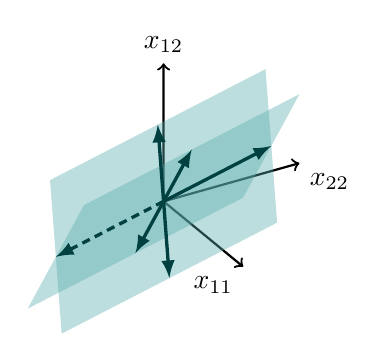
\begin{tikzpicture}%
                    [x={(0.505216cm, -0.414953cm)},
                    y={(0.862993cm, 0.242833cm)},
                    z={(0.000089cm, 0.876839cm)},
                    scale=1,%3.33000000,
                    back/.style={loosely dotted, thin},
                    edge/.style={color=teal!50!black, thick},
                    facet1/.style={fill=teal!65!white,fill opacity=0.400000}]
                %% Drawing the axes
                \draw[color=black,thick,->] (0,0,0) -- (2,0,0) node[anchor=north east]{$x_{11}$};
                \draw[color=black,thick,->] (0,0,0) -- (0,2,0) node[anchor=north west]{$x_{22}$};
                \draw[color=black,thick,->] (0,0,0) -- (0,0,2) node[anchor=south]{$x_{12}$};
                %%
                %% Drawing the interior
                %%
                \fill[facet1] (0, 0, 0) -- (1,-0.5,-0.5) -- (0,-1.5,-1.5) -- (-1,-1,-1) -- (0, 0, 0) -- cycle {};
                \fill[facet1] (0, 0, 0) -- (1,-1,0) -- (0,-2,-1) -- (-1,-1,-1) -- (0, 0, 0) -- cycle {};
                \fill[facet1] (0, 0, 0) -- (1,-0.5,-0.5) -- (2,0.5,0.5) -- (1,1,1) -- (0, 0, 0) -- cycle {};
                \fill[facet1] (0, 0, 0) -- (1,-1,0) -- (2,0,1) -- (1,1,1) -- (0, 0, 0) -- cycle {};
                \fill[facet1] (0, 0, 0) -- (-1,0.5,0.5) -- (-2,-0.5,-0.5) -- (-1,-1,-1) -- (0, 0, 0) -- cycle {};
                \fill[facet1] (0, 0, 0) -- (-1,0.5,0.5) -- (0,1.5,1.5) -- (1,1,1) -- (0, 0, 0) -- cycle {};
                \fill[facet1] (0, 0, 0) -- (-1,1,0) -- (-2,0,-1) -- (-1,-1,-1) -- (0, 0, 0) -- cycle {};
                \fill[facet1] (0, 0, 0) -- (-1,1,0) -- (0,2,1) -- (1,1,1) -- (0, 0, 0) -- cycle {};
                
                %% Rays for normal cones:   
                \draw[color=teal!50!black,very thick,-latex] (0,0,0)--(1,-0.5,-0.5);
                \draw[color=teal!50!black,very thick,-latex] (0,0,0)--(1,-1,0);
                \draw[color=teal!50!black,very thick,-latex] (0,0,0)--(-1,1,0);
                \draw[color=teal!50!black,very thick,-latex] (0,0,0)--(-1,0.5,0.5);
                \draw[color=teal!50!black,very thick,-latex] (0,0,0)--(1,1,1);
                \draw[densely dashed, color=teal!50!black,very thick,-latex] (0,0,0)--(-1,-1,-1);
                \end{tikzpicture}
            \end{center}\centering \footnotesize{Normal fan to $P_2$}
    \end{column}
\end{columns} 

\end{frame}
\end{document}